% !TEX TS?program = pdflatexmk
\documentclass{article}
\usepackage[utf8]{inputenc}
\usepackage{graphicx}
\usepackage{amssymb, amsmath, amsthm}
\usepackage{bbm}
\usepackage{biblatex}
\usepackage{floatrow}
\usepackage{tabu}
\newfloatcommand{capbtabbox}{table}[][\FBwidth]
\addbibresource{references.bib}
\newcommand\numberthis{\addtocounter{equation}{1}\tag{\theequation}}
\usepackage[margin=1in]{geometry}
\usepackage{siunitx}
\usepackage{float}
\usepackage{verbatim}
\graphicspath{ {report_figures/} }
\parskip = 0.1in

\begin{document}
\title{Analysis of Precipitation in the Northwestern United States}
\author{Matthew Wiens\footnote{Lived in Seattle for 15 years}, Kelly Kung}
\date{December 21, 2017}
\maketitle
\begin{abstract}

Predicting precipitation is a key problem for residents of the Pacific Northwest, from its impact on family vacations to landslides. A noteworthy feature of the area is distinct chances of precipitation between the summer and winter due to the topographical differences. There have been previous research regarding precipitation differences in the Northwest, but there is room to build upon their results. In this report, we adopt a Bayesian methodology in order to obtain predictive results and propose two models for differentiating the two seasons and understanding the chance of rain across different climatic areas of the state. The first involves examining the start dates of each season and the second looks at the probability of rain on a given day. Using these models, we find that regions to the west of the Cascade Mountains have generally earlier and longer summers than in the eastern regions, but the eastern regions are generally drier. With these results, we can better understand the precipitation patterns of the areas and can predict optimal times to travel from a rainy region to a dry region. 

\end{abstract}

\section{Introduction}

Residents and visitors to the Pacific Northwest (Oregon and Washington) notice a distinct pattern year over year: most days are rainy during the winter, and then they feel that there a distinct point during the spring or early summer when the weather becomes mostly dry. During early fall, the nice weather switches back to rain.  However, the timing of the switch varies throughout the area, with the prominent Cascade Mountains being a key factor. There are many resorts on the east side of the Cascade Range that cater to residents of the west side looking to escape the rain. 

Widmann and Bretherton\footnote{M. Widmann and C. S. Bretherton. Validation of Mesoscale Precipitation in the NCEP Reanalysis Using a New Gridcell Dataset for the Northwestern United States. In Journal of Climate, 13(11), 1936-1950. 2000.} developed a methodology to control for local variation in topography and precipitation data and generated a dataset containing 46 years of estimated precipitation data in a 50km by 50km grid.  In comparison, general models of atmospheric weather operate on the order of hundreds of kilometers, so there is significant room to improve the spatial resolution of weather models.  In particular, local topographic features are not captured by general models, which is a limitation in regions like the Pacific Northwest. The temporal and spatial correlation is also highly dependent on the topography and are difficult to model, and therefore there has been a focus on parametrizing models and reducing the dimensionality. 

In this report, we analyze the precipitation differences using a Bayesian approach for two reasons: first, to capture prior beliefs  from living in the area of one author, and second to be able to discuss distributions around complicated model parameters and probabilistic beliefs about the state of weather on a specific day of the year. Bayesian approaches for daily precipitation data are not new, for example in Olson and Kleiber's work.\footnote{B. Olson and W. Kleiber. Approximate Bayesian computation methods for daily spatiotemporal precipitation occurrence simulation,Water Resour. Res., 53, 3352?3372,doi:10.1002/2016WR019741. 2017.} With a Bayesian approach, we hope to model (1) the beginning of dry and wet seasons and (2) the probability of precipitation in the different areas. These models will provide us with tools in order to further analyze and understand the precipitation patterns in the Northwest. 

This report is organized as follows. In Section 2, we refine our goals with our analysis, which motivates the creation of several variables in our dataset, which is also outlined in the same section. In Section 3, we discuss the two models that we used in order to analyze the data.  We then begin our analysis of the dataset in Section 4, and in Section 5, we conclude our report with summaries of our analysis as well as potential future directions.

\section{Background}

%The general problem we're trying to model
\subsection{Main Goals of Analysis}
In their analysis, Widmann and Bretherton found that there was some variability in precipitation levels in the different topographical areas in the Northwestern United States. For this report, we further investigate the variability in the different areas in order to build upon their results. In particular, we are interested in analysis regarding when the dry and wet seasons start and the probability of rain on a given day. By using a Bayesian approach, we are able to calculate posterior probabilities in order to conduct further analysis and answer more questions. For example, which area has the longest summer? Which area is most likely to have the latest winter?  What is the chance that someone can escape the bad weather by traveling to another part of the are? With our models and analysis, we may be able to better understand the precipitation patterns in the different topographical areas of the Pacific Northwest. 

\subsection{Precipitation Dataset}
%Our Data
To analyze the precipitation in the Pacific Northwest, we use the dataset generated by Widmann and Bretherton. This data contains 46 years\footnote{Note that when creating the indicators for years, we did not take into account of leap years, which resulted in data points that spilled over to the next year. We just take the years in which we have a year's worth of data for.} of precipitation logs (measured in millimeters) from 1949 - 1994 that was collected form the National Weather Service and was corrected by the National Climatic Data Center\footnote{The data was corrected during the 'Validated Historical Daily Data' project, which aimed to verify the data collected.}\footnote{T. Reek, S. Doty, and T. Owen. A Deterministic Approach to the Validation of Historical Daily Temperature and Precipitation Data from the Cooperative Network. In Bulletin of the American Meteorological Society 73, no. 6: 753-62. 1992.}. The dataset is a 3-dimensional array with a 2-dimensional 16 (latitude) by 17 (longitude) grid cell\footnote{Each cell represents an area approximately 50km by 50km.} for each of the 16,801 days. However, there are approximately 32,000 missing values which correspond to areas with few functional weather stations, such as the ocean and some areas in the southeast. Using this dataset, we then transform and create several variables in order to obtain a model to analyze the precipitation. 

\subsection{Grouping of Areas} \label{GroupArea}
%Discussion of the areas
The Pacific Northwest has a varied climate, from temperate rainforests on the Pacific coast to desert in Southeastern Oregon, which has a major impact on the seasons. Therefore, each grid cell is classified into one of nine climatic zones as follows:
\begin{enumerate}
\item Washington Coastline (Temperate Rainforest)
\item Oregon Coastline
\item Western Washington / Seattle Metropolitan Area
\item Portland Metropolitan Area / Willamette Valley / Southwestern Oregon
\item Cascade Range
\item Columbia Plateau
\item Selkirk Mountains
\item Blue Mountains
\item Eastern Oregon / High Desert / Great Basin
\end{enumerate}

These zones are decided by considering average precipitation over the time period of the data and the topographic features of the region (Figure \ref{fig:topo}). In general, the regions correspond to areas with similar topography. For example, region 8, corresponds to the mountain range in northeastern Oregon, which extends into Idaho. However, only data from Oregon is considered. The rainfall for the region was aggregated by considering if there was measurable precipitation (more than 0.1 mm) in each grid by day, and then for each day, if the majority of grid cells reported precipitation, then a value of \textit{rain} was assigned to the area, else it was \textit{dry}.


\begin{figure}[h!]
\centering
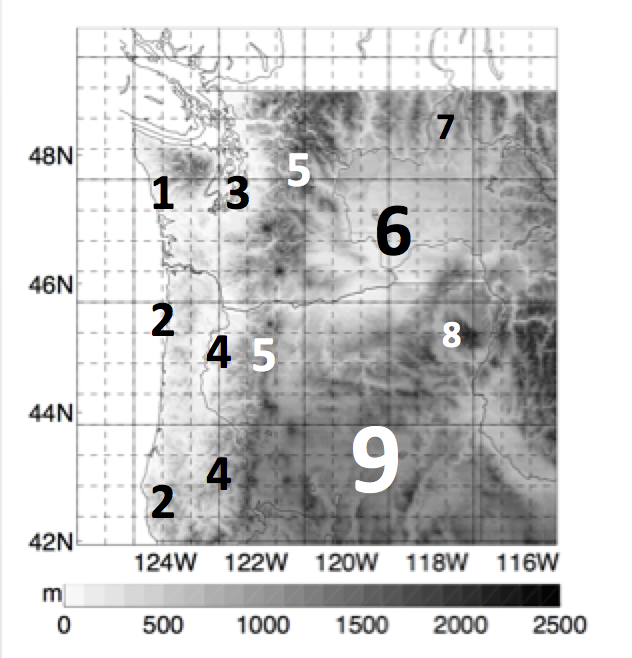
\includegraphics[width = .4\textwidth, height = 6cm]{LabledTopography}
\caption{Topography of the Pacific Northwest, with the 9 areas indicated }
\label{fig:topo}
\end{figure}


\subsection{Indicators for Dry and Wet Season}
Using the area groups and daily precipitation indicators, mentioned in Section \ref{GroupArea}, we then proceeded to create indicators of when the dry season and wet season starts. To do this, we create an algorithm that chooses indicators of start days for  the dry season ($X_{min}$) and wet season ($X_{max}$) such that it maximizes the number of \textit{dry} days in the dry season and maximizes the number of \textit{wet} days in the wet season, with the weights determined by the overall prevalence of dry and wet days. I.e., if there are only a few dry days in the year, such as in area 1, the algorithm puts more weight on classifying the dry days correctly. For example, we expect $X_{min}$ to be approximately 170 and $X_{max}$ to be approximately 260 because these dates correspond to the beginning of summer and the beginning of autumn. Using this algorithm, we find the start dates for the dry and wet seasons for each region for the 46 years.


\section{Modeling}
\subsection{Multivariate Normal Model}
Our first model is motivated by the goal of determining when the dry and wet seasons start. We model each of the start dates using a semi-conjugate multivariate normal prior and multivariate normal likelihood. We choose this model because it has a closed form and we are able to sample from the posterior distribution using a Gibbs sampler on the full conditionals. Furthermore, upon initial exploration of the data, we see that the distribution of both the start dates of dry and wet seasons are approximately normal as seen in Figure \ref{PDXexample}. Thus, we continue with the multivariate normal likelihood with confidence that it represents the data we have. 

\begin{figure}[H]
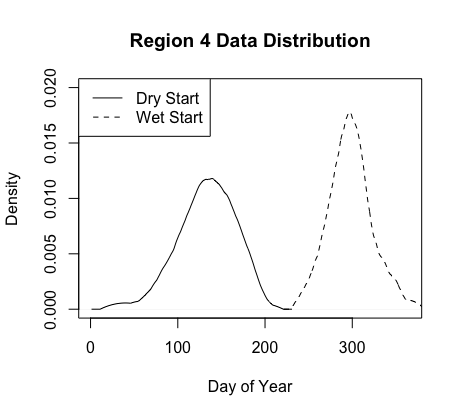
\includegraphics[width = .4\textwidth, height = 6cm]{Area4DataDistribution}
\caption{Kernel Density Estimate of the start and end of the dry season for Portland}
\label{PDXexample}
\end{figure}

We first define the semi-conjugate prior distributions as follows. 

\begin{align*}
\theta \sim MVN(\mu_0, \Lambda_0) \\
\Sigma \sim Inverse-Wishart_{\nu_0}(\Sigma_0^{-1})
\end{align*}

To determine the prior parameters, we let $\mu_0 = \begin{bmatrix} X_{min} \\ X_{max} \end{bmatrix} = \begin{bmatrix} 170 \\ 260 \end{bmatrix}$ and $\Lambda_0 = \begin{bmatrix} 30^2 & 0 \\ 0 & 30^2 \end{bmatrix}$ for all 9 area groups. The prior means are chosen according to when the summer and autumn season starts and the prior standard deviations of the $\theta 's$ were chosen to represent a spread of one month. To set the prior parameter for $\Sigma$, we choose the $\Sigma_0$ values by mimicking the methods used during our homework, where we let $\Sigma_0$ equal the \textit{variance - covariance} matrices for each area group from the data. The parameters for $\Sigma_0$ of the nine regions are shown in Table \ref{tab:sigmavals}. We also let $\nu_0 = 2$ in order to have a relative non-informative prior.

\begin{table}[h!]
\centering
\renewcommand{\arraystretch}{1}

\begin{tabular}{|*5{>{\renewcommand{\arraystretch}{1}}c|}}
\hline
\textbf{1} & \textbf{2} & \textbf{3} & \textbf{4} & \textbf{5}\\
\hline
$\left[ \begin{array}{cc} 1154.93 & 179.97  \\ 179.97 & 618.95 \end{array}\right]$ & $\left[ \begin{array}{cc} 658.26 & 134.48 \\ 134.48 & 423.75  \end{array}\right]$ & $\left[ \begin{array}{cc} 1006.46 & 115.78 \\ 115.78 & 434.10  \end{array}\right]$ & $\left[ \begin{array}{cc} 1000.96 & 87.99 \\ 87.99 & 575.44  \end{array}\right]$ & $\left[ \begin{array}{cc} 993.37 & 236.99 \\ 236.99 & 405.11  \end{array}\right]$ \\
\hline
\end{tabular}

\bigskip

\begin{tabular}{|*4{>{\renewcommand{\arraystretch}{1}}c|}}
\hline
\textbf{6} & \textbf{7} & \textbf{8} & \textbf{9}\\
\hline
$\left[ \begin{array}{cc} 2943.59 & 630.29 \\ 630.29 & 728.15  \end{array}\right]$ & $\left[ \begin{array}{cc} 3574.88 & 884.72 \\ 884.72 & 874.46  \end{array}\right]$ & $\left[ \begin{array}{cc} 2221.71 & 210.85 \\ 210.85 & 500.14  \end{array}\right]$ & $\left[ \begin{array}{cc} 1974.74 & 250.49 \\ 250.49 & 684.75  \end{array}\right]$ \\
\hline
\end{tabular}
\caption{Table of prior $\Sigma_0$ values for each area group}
\label{tab:sigmavals}
\end{table}



In order to conduct Gibbs sampling, we need full conditionals of $\theta$ and $\Sigma$, which are shown below. By running Gibbs sampling on these full conditionals, we are effectively sampling from the posterior distribution and so we can obtain posterior estimates of $\theta$ and $\Sigma$.
\begin{align}
\theta | \Sigma, y \sim MVN(\mu_n(\Sigma), \Lambda_n(\Sigma)))  \nonumber \\
\Sigma | \theta, y \sim Inverse - Wishart_{\nu_n} (\Sigma_n^{-1}(\theta)) \nonumber \\
\nonumber \\
\mu_n(\Sigma) =(\Lambda_0^{-1} + n\Sigma^{-1})^{-1}(\Lambda_0^{-1}\mu_0 + n\Sigma^{-1}\bar{y}) \nonumber \\
\Lambda_n^{-1}(\Sigma) = \Lambda_0^{-1} + n\Sigma^{-1} \nonumber \\
\nu_n = \nu_0 + n \nonumber \\
\Sigma_n(\theta) = \Sigma_0 + \sum_{i=1}^n(y_i - \theta)(y_i - \theta)^T \nonumber
\end{align}

\subsection{Daily Precipitation Chance Model}
%Maybe discuss first model here? It worked pretty well and informed future direction

We further develop our analysis by considering the probability of precipitation on each day for the summer (dry) and winter (rainy) seasons. This is motivated by the idea of trying to plan outdoor activities in each area of the Pacific Northwest and deciding if there is value in traveling to a different area to escape rain.
Therefore, the following model is proposed based on the observed V shape of the probability of precipitation by day as in Figure \ref{fig:area4}:
\begin{itemize}
\item The data is binary data representing if it rained or not for each day of the year
\item The probability of rain on the jth day of the year is given by the following piecewise linear function: $\pi_j = \theta_0 + (a * 1_{j < \theta^*} + b*1_{j>=\theta^*})(j - \theta^*)$
\item $\theta_0$ can be interpreted as the chance of precipitation on the driest day of the year, $\theta^*$ is the day number of the driest day, and $a$ and $b$ are the slopes of the springtime daily change in precipitation chance, and fall daily change in precipitation chance, respectively
\item Observing precipitation on the $jth$ day of the year is a Bernoulli random variable, with parameter $\pi_j$
\end{itemize}

Furthermore, we note the wintertime (January - March) is has a constant, large chance of rain across the region, as seen in Figure \ref{fig:area4}, and therefore we choose to focus our analysis on the periods where this chance is changing. 
We use weakly informative priors in this model: $\theta_0 \sim N(210,900)$,$\theta^* \sim \beta(5,20)$, $b \sim -a \sim N(.004,.002^2)$. These priors capture the prior beliefs that the driest days are around the end of July, and we're very sure they're within a two months on either side, and that the driest days have about a 20\% chance of rain. 
The slopes follow from noting that the rainiest part of the year has about a 80\% chance of rain, and choosing a slope that appropriately interpolates the wettest and driest portions of the year, and choose the variance such that there is only a small chance that the sign of each portion of the slope is contrary to our expectations.
The likelihood and full conditionals of the parameters for this model exist in closed form, however they are not informative, so we proceed to use a Metropolis MCMC algorithm to produce posterior distributions.

\begin{figure}[h!]
\centering
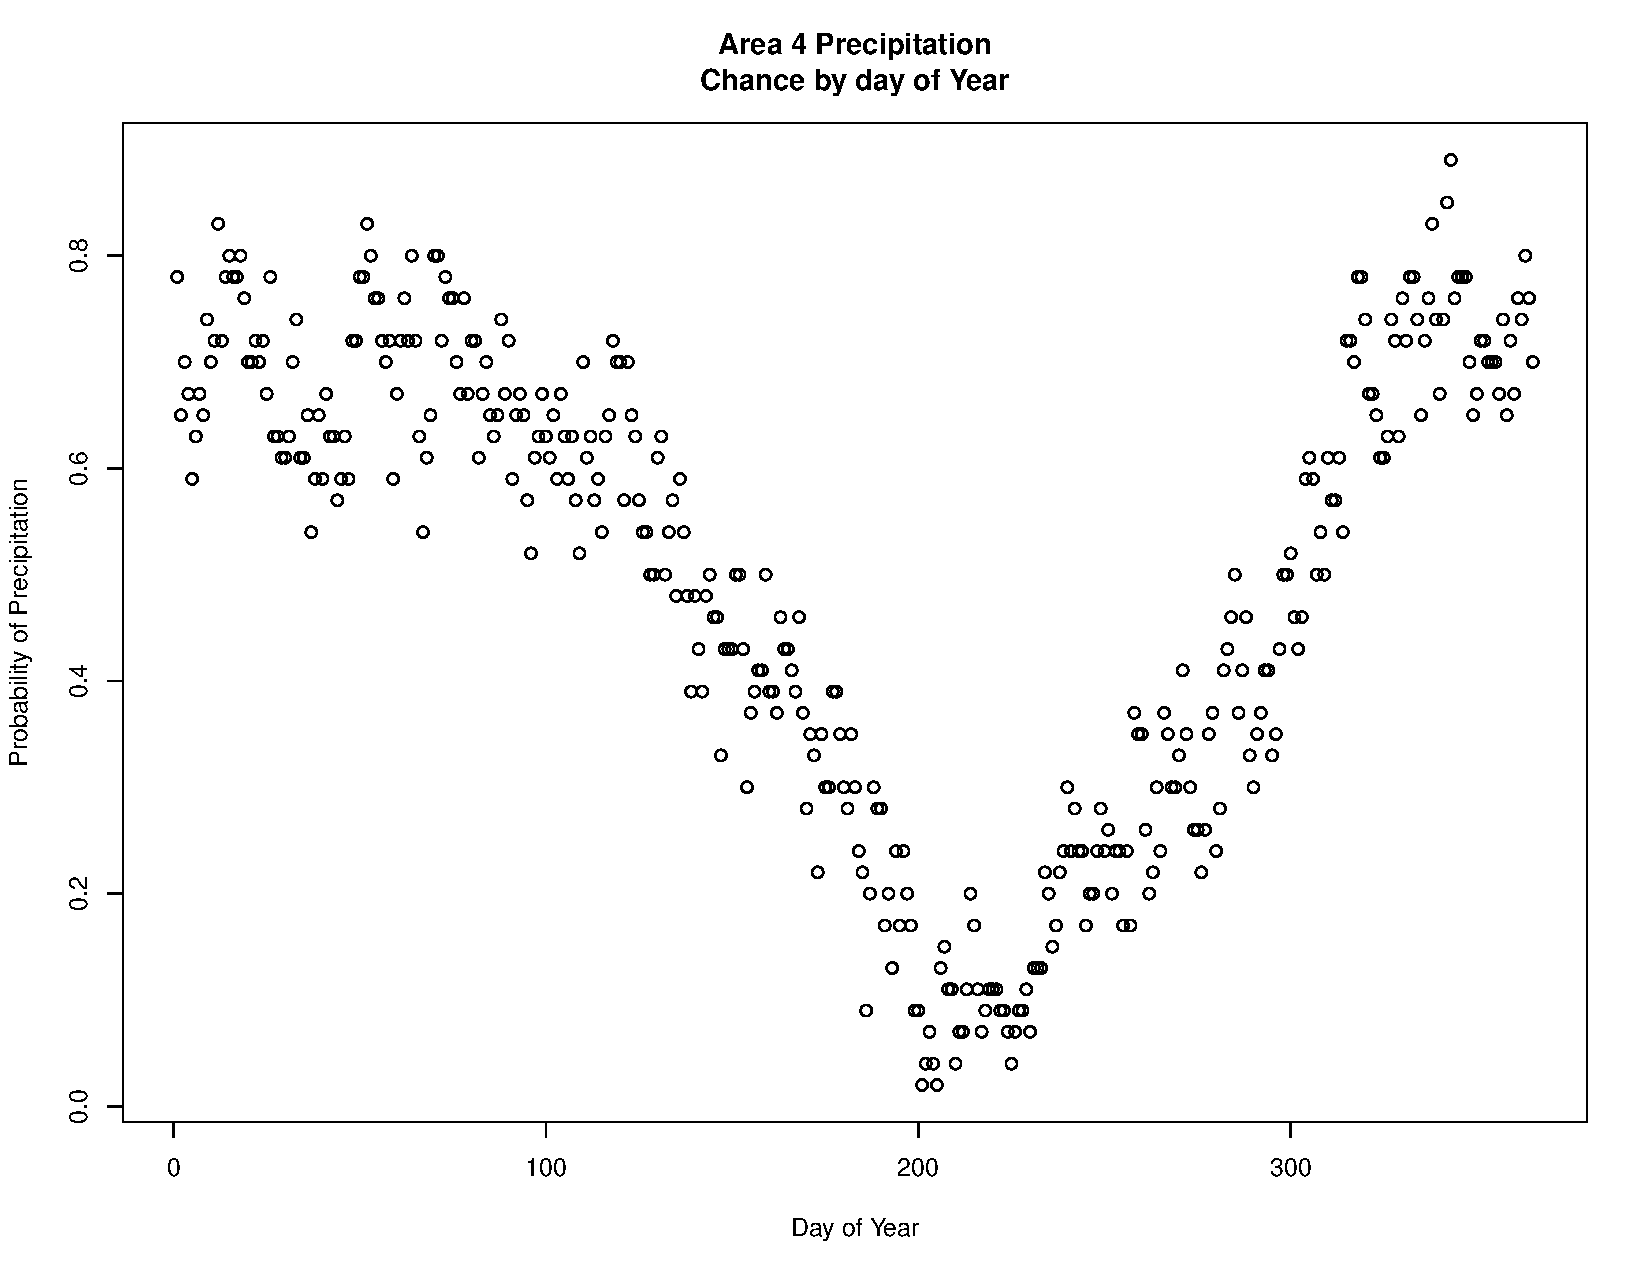
\includegraphics[width = .4\textwidth, height = 6cm]{Area4PrecipByDay}
\caption{Western Oregon precipitation chance over the year}
\label{fig:area4}
\end{figure}
%Put in analytical results here


\section{Analysis}

\subsection{Multivariate Normal Model}
Using the semi-conjugate multivariate normal model described in section 3.1, we used a Gibbs sampler to generate samples from the posterior distributions of $\theta$ and $\Sigma$ as well as the posterior predictive distribution $\begin{bmatrix} X_{min} \\ X_{max} \end{bmatrix}  \sim MVN(\theta, \Sigma)$. When drawing samples from the posterior predictive distribution, we used the restriction: $(X_{min} ,X_{max}) \epsilon (0,365)$ to ensure that the sampled data points represents dates in a year. Because we used Gibbs sampler, we needed to take into account of the dependencies of the Markov Chains. This is important because issues may arise if the chain is stuck in one area of the distribution because of the previous sample. To account for these dependencies, we ran 20,000 simulations in order to obtain high effective sizes. On average, the effective sizes were: $\theta_{X_{min}} : 10,795,  \theta_{X_{max}}: 7,229, \Sigma_{X_{min}}: 11,286, \Sigma_{X_{max}}: 8,906$. We then examined the autocorrelation plots and saw that it was fairly high, especially for the lag periods of 1 and 2 iterations. To resolve this issue, we thinned out the data by taking every tenth entry which resulted in 2,000 sampled values. Figure \ref{acfPlot} shows the autocorrelation plots before and after thinning the data. We then analyzed the data using this thinned out dataset.

\begin{figure}[H]
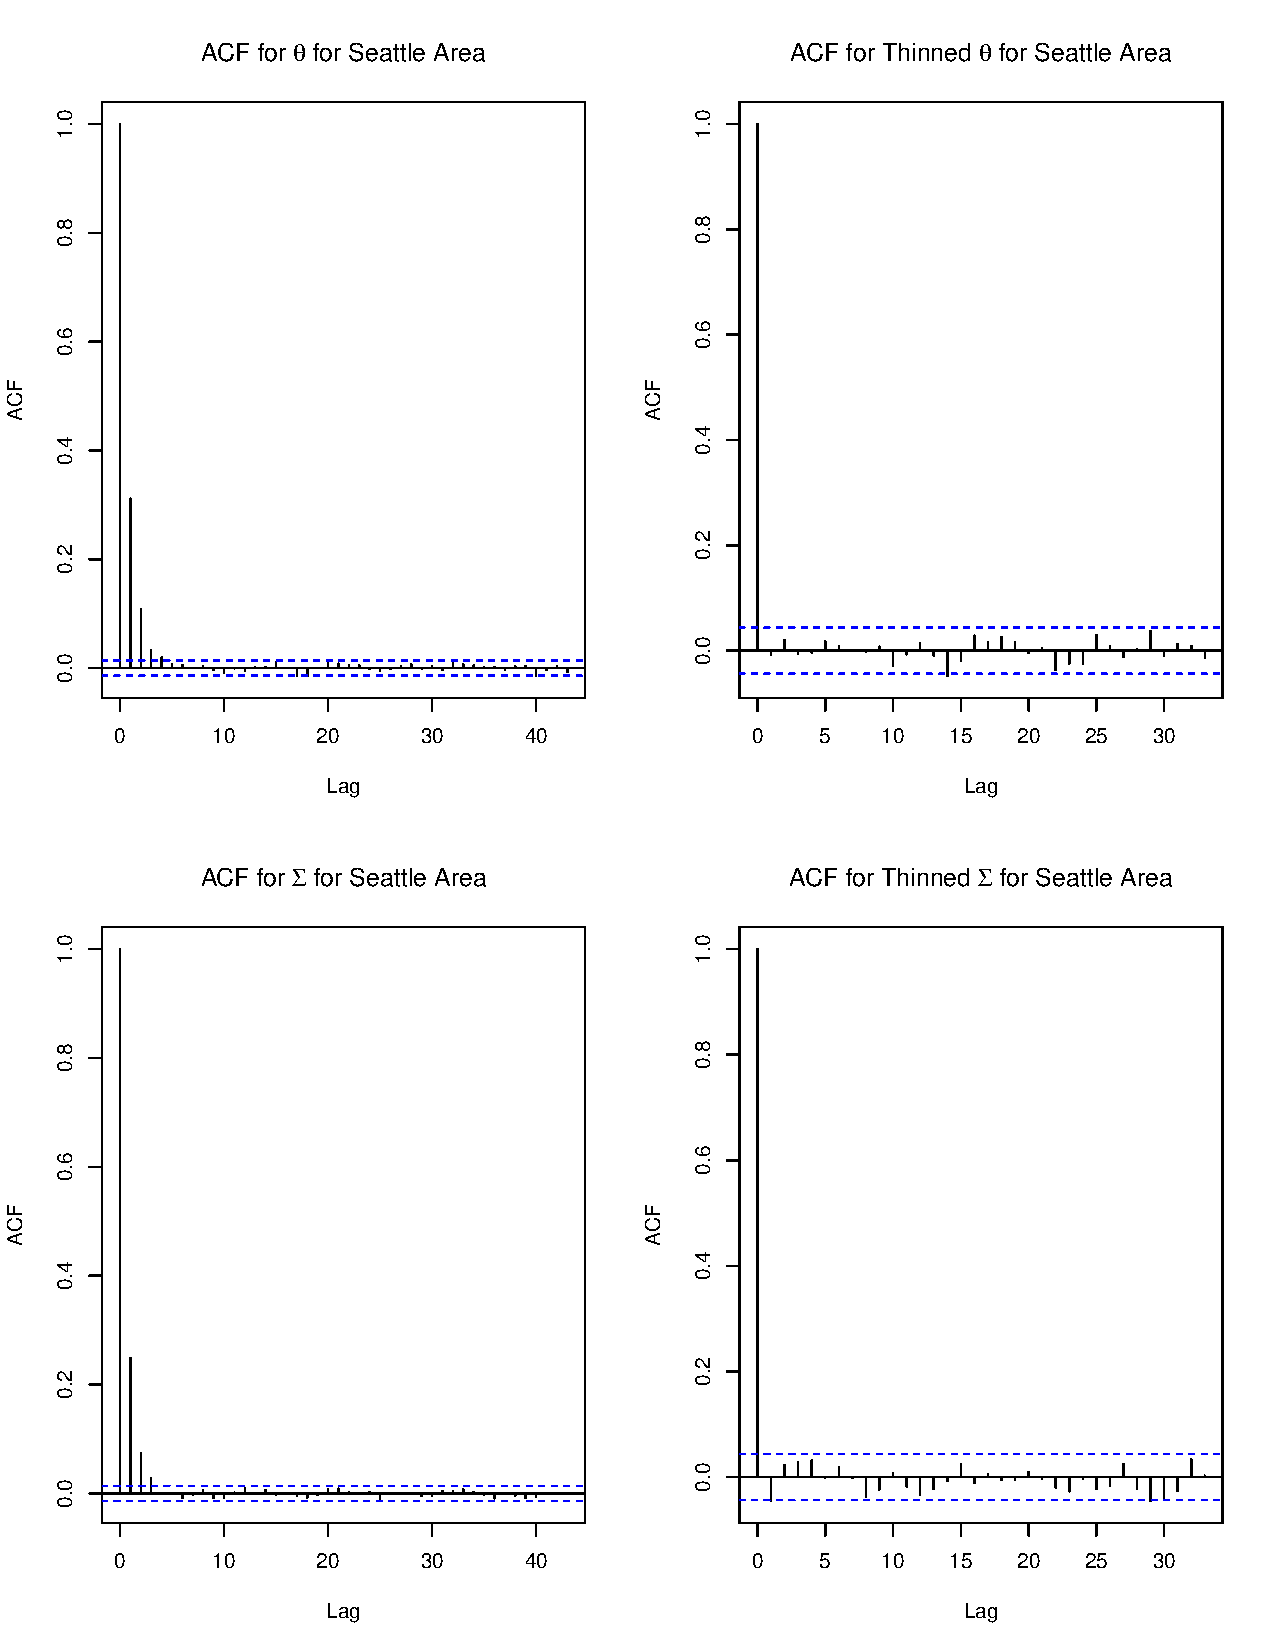
\includegraphics[width = .6\textwidth, height = 7cm]{acfplots}
\caption{Autocorrelation plots for parameters before and after thinning data}
\label{acfPlot}
\end{figure}

We report summary statistics of $\theta$, the posterior mean of the start date of the dry and west seasons, in Table \ref{tab:meanparams}.  In particular we note the variability in the mean start dates of the dry season between the regions, which ranges from 149 - 162, and the increase in the mean start date as we move towards the eastern regions. On the other hand, the end date of the dry season is much more consistent across regions, ranging from 280 to 289. This suggests larger weather patterns triggering the end of the dry season, which are consistent between years. %expand on this last though? 

\begin{table}[h!]
\begin{tabular}{|l|c|c|c|c|}
\hline
Region & Start Date Mean & Start Date Variance & End Date Mean & End Date Variance\\
\hline
\hline
1&152&24&280&17\\
2&149&20&288&18\\
3&153&22&284&15\\
4&154&23&282&22\\
5&153&17&289&12\\
6&158&30&283&27\\
7&158&28&284&28\\
8&162&25&289&20\\
9&160&26&284&30\\
\hline
\end{tabular}
\caption{Posterior Mean and Variance of $\theta$}
\label{tab:meanparams}
\end{table}

Using the predictive posterior sample, we also generated probabilities that an area has the earliest dry season and latest wet season in a given year. The probabilities are shown in Table \ref{lengthProb}. Looking at the probabilities, we see that the region 6 and 7 (Columbia Plateau and Selkirk Mountains) are most likely to have the earliest dry season and latest wet season. This aligns with the climate of the area since the Columbia Plateau is somewhat arid because of the rain shadow of the Cascade Range and the Selkirk Mountains are located in the generally drier, East. Since the two regions are relatively close to each other, it makes sense that they share the same precipitation patterns. However, neighboring regions, such as region 5, the Cascade Range, have fairly low probabilities of having the earliest dry season. This suggests that the precipitation patterns do vary across the Northwest region, and it is likely due to the topographical makeup of each area. This is because although the Cascade Range and Columbia Plateau are only approximately 320 km apart, the Cascade Range does not share similar patterns as the Columbia Plateau and Selkirk Mountains which suggests that there is another underlying reason for the differences in precipitation patterns. 

Looking at the lengths of the dry season in Table \ref{lengthProb}, there is quite some variability, with a difference of 20 days of the longest and shortest periods.  The Oregon Coastline (region 2) and Cascade Range (region 5) have the longest dry season while region 9 (Eastern Oregon border area) has the shortest dry season. Although this is not as we first expected, it makes sense according to how we defined the start dates and the climate of the regions. In the western regions, we expected a clear distinction between the dry and wet seasons whereas the eastern regions are generally drier and may not have a clear distinction of the two seasons. Therefore, we are most likely distinguishing between \textit{very dry} days from the normally \textit{dry} days in areas such the Columbia Plateau, Selkirk Mountains, and the desert/basin area. Thus, we are essentially comparing the lengths of  very dry seasons in the eastern regions and dry seasons in the western regions, which may be an explanation of the results.  However, the results still lead us to believe that there are varying precipitation patterns across the regions.

\begin{table}[h!]
\begin{tabular}{|l|c|c|c|}
\hline
Region & Earliest Dry Season & Latest Wet Season & Length of Dry Season\\
\hline
\hline
1&0.099&0.074&129 \\
2&0.074&0.032&138 \\
3&0.091&0.057&122 \\
4&0.087&0.081&127\\
5&0.073&0.068&136 \\
6&0.180&0.198&123\\
7&0.179&0.200&121\\
8&0.109&0.145&129\\
9&0.110&0.147&119\\
\hline
\end{tabular}
\caption{Area with probabilities of earliest and latest start times as well as length of dry season }
\label{lengthProb}
\end{table}


\subsection{Daily Precipitation Chance Model}

The model described in section 3.2 was implemented with a Metropolis MCMC algorithm for each of the nine areas, with a thinning by a factor of 50 to reduce autocorrelation. Each of the nine areas was again treated independently, because at the scale of which we defined the regions, there is minimal correlation in daily precipitation.  As expected, the driest day of the year in all the regions is in early August. All the regions on the west side of the Cascade Range had the driest day around day number 220, while those east of the mountains had the driest day around day number 230, which analogous to the results from the first model we explored and reported in Table \ref{tab:meanparams}. These posterior distributions are reported in Figure \ref{fig:driestDist}, and it highlights the clear difference between the two geographical areas. However, the chance of rain on the driest day of the year varied significantly more. In region 1, the temperate rainforest and coast, the minimum chance was 25\%, while in region 9, which contains part of the Great Basin and other steppe climates, the minimum chance was 6\%. The estimated chance of rain for each day and each region is reported in Figure \ref{fig:9by9}.

\begin{figure}
\centering
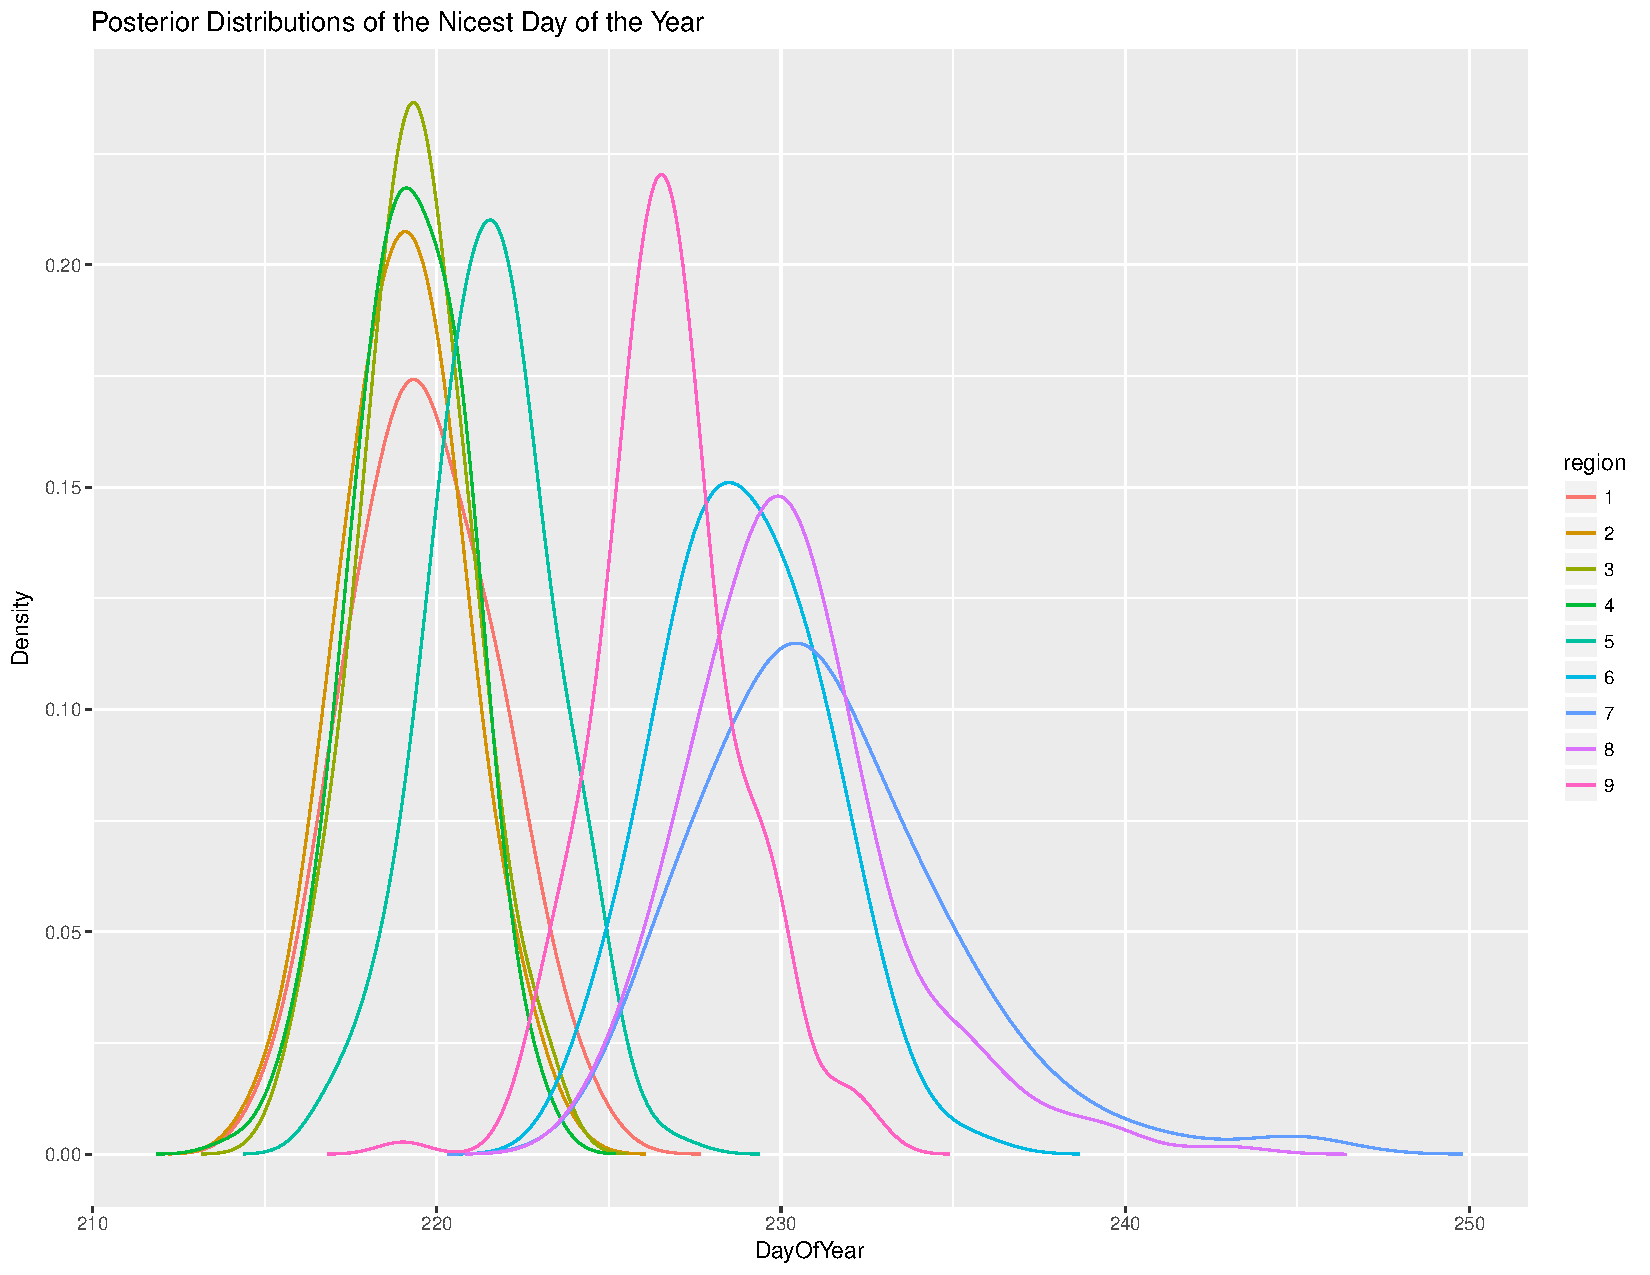
\includegraphics[width = .4\textwidth, height = 6cm]{NicestDayOfYear}
\caption{Distributions of the day with minimum chance of rain}
\label{fig:driestDist}
\end{figure}



\begin{figure}[h!]
\centering
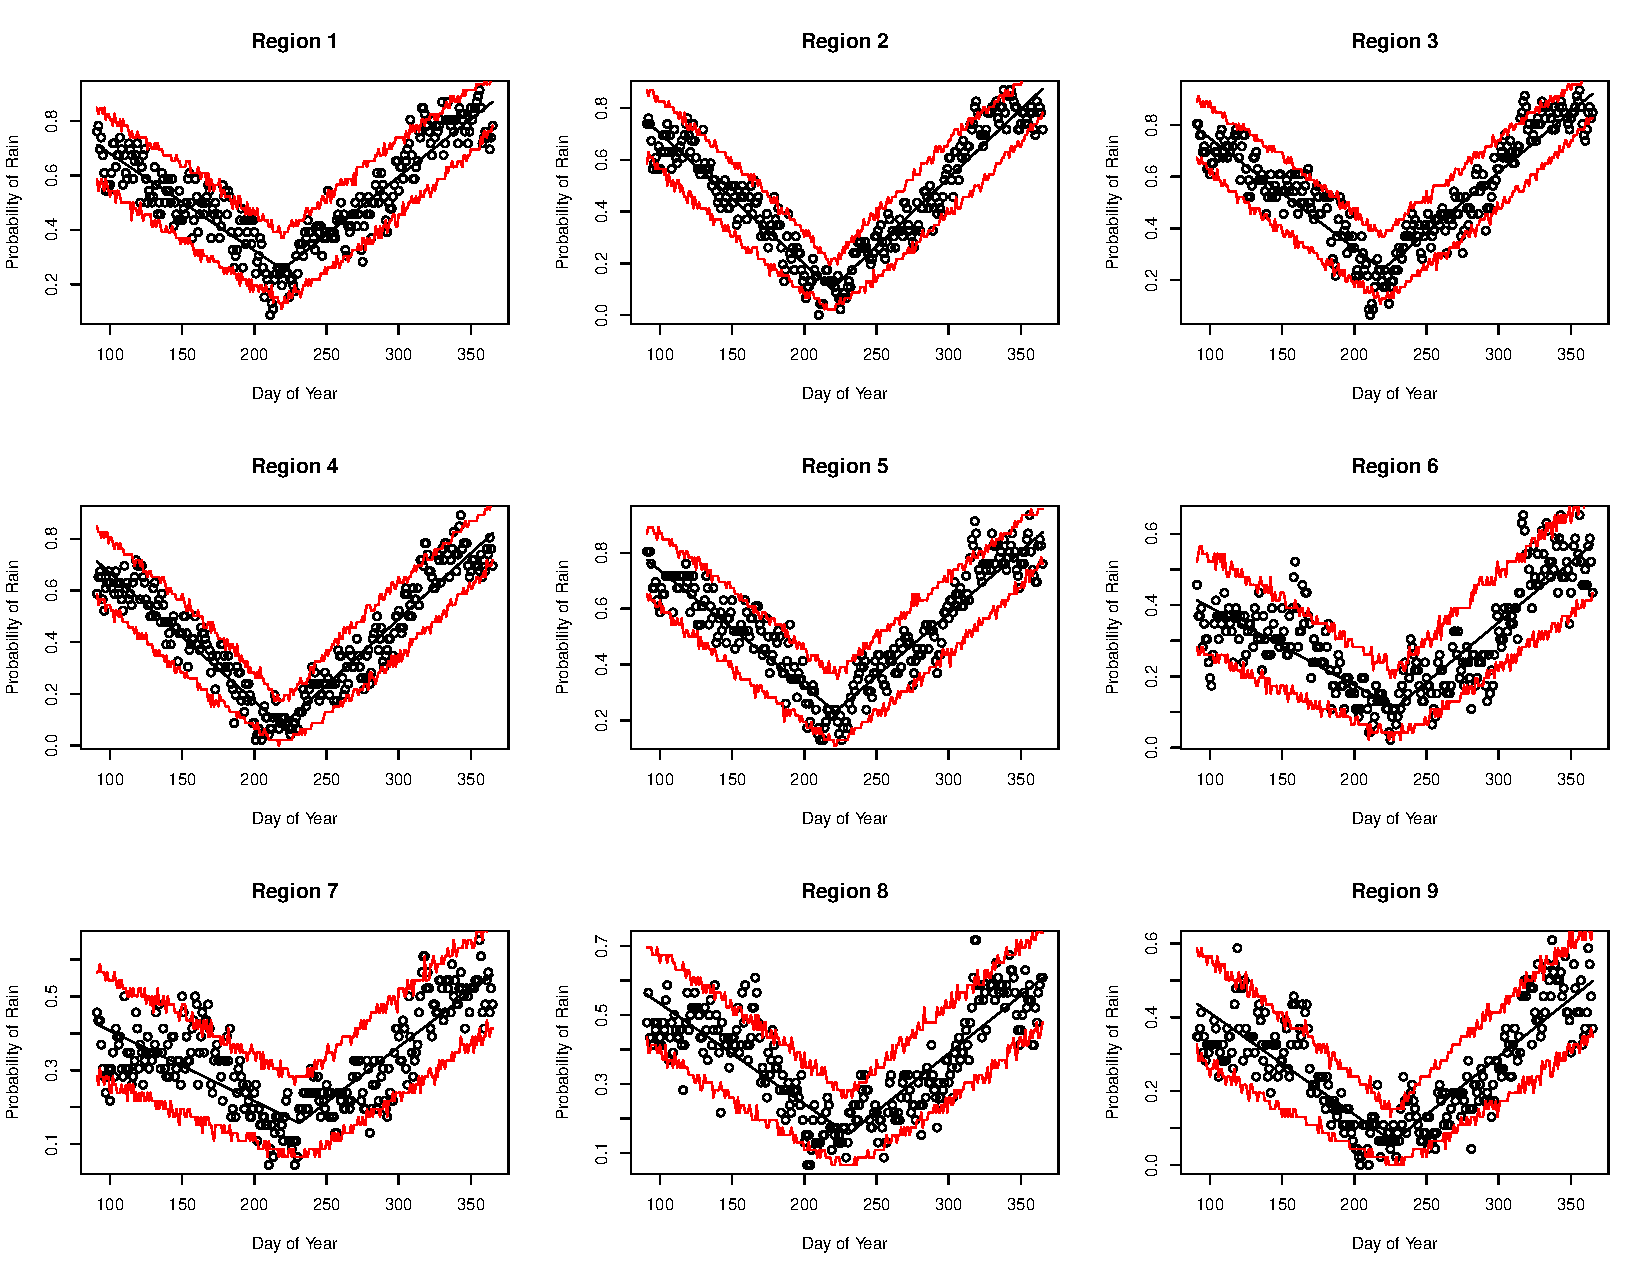
\includegraphics[width = .8\textwidth, height = 12cm]{AllRegionPosterior}
\caption{Data Points for each region, with mean estimate and 95\% credible interval for the observed chance of rain over 46 years. In most regions, approximately 95\% of the data is inside the credible interval, indicating a valid model}
\label{fig:9by9}
\end{figure}
Posterior estimates of the mean of the slopes are all between 0.003 and 0.006 for the fall, and the negative, but the same range for the springtime. The natural interpretation is that for each day that passes, the probability of rain changes by 0.3\% to 0.6\%. However, there is little correlation of the means (-0.07) between how dry the driest day is, and how rapidly the chance of precipitation changes. We suspect that this is due to the variety of topographical features that obscure any correlation. 

\begin{figure}[H]
\centering
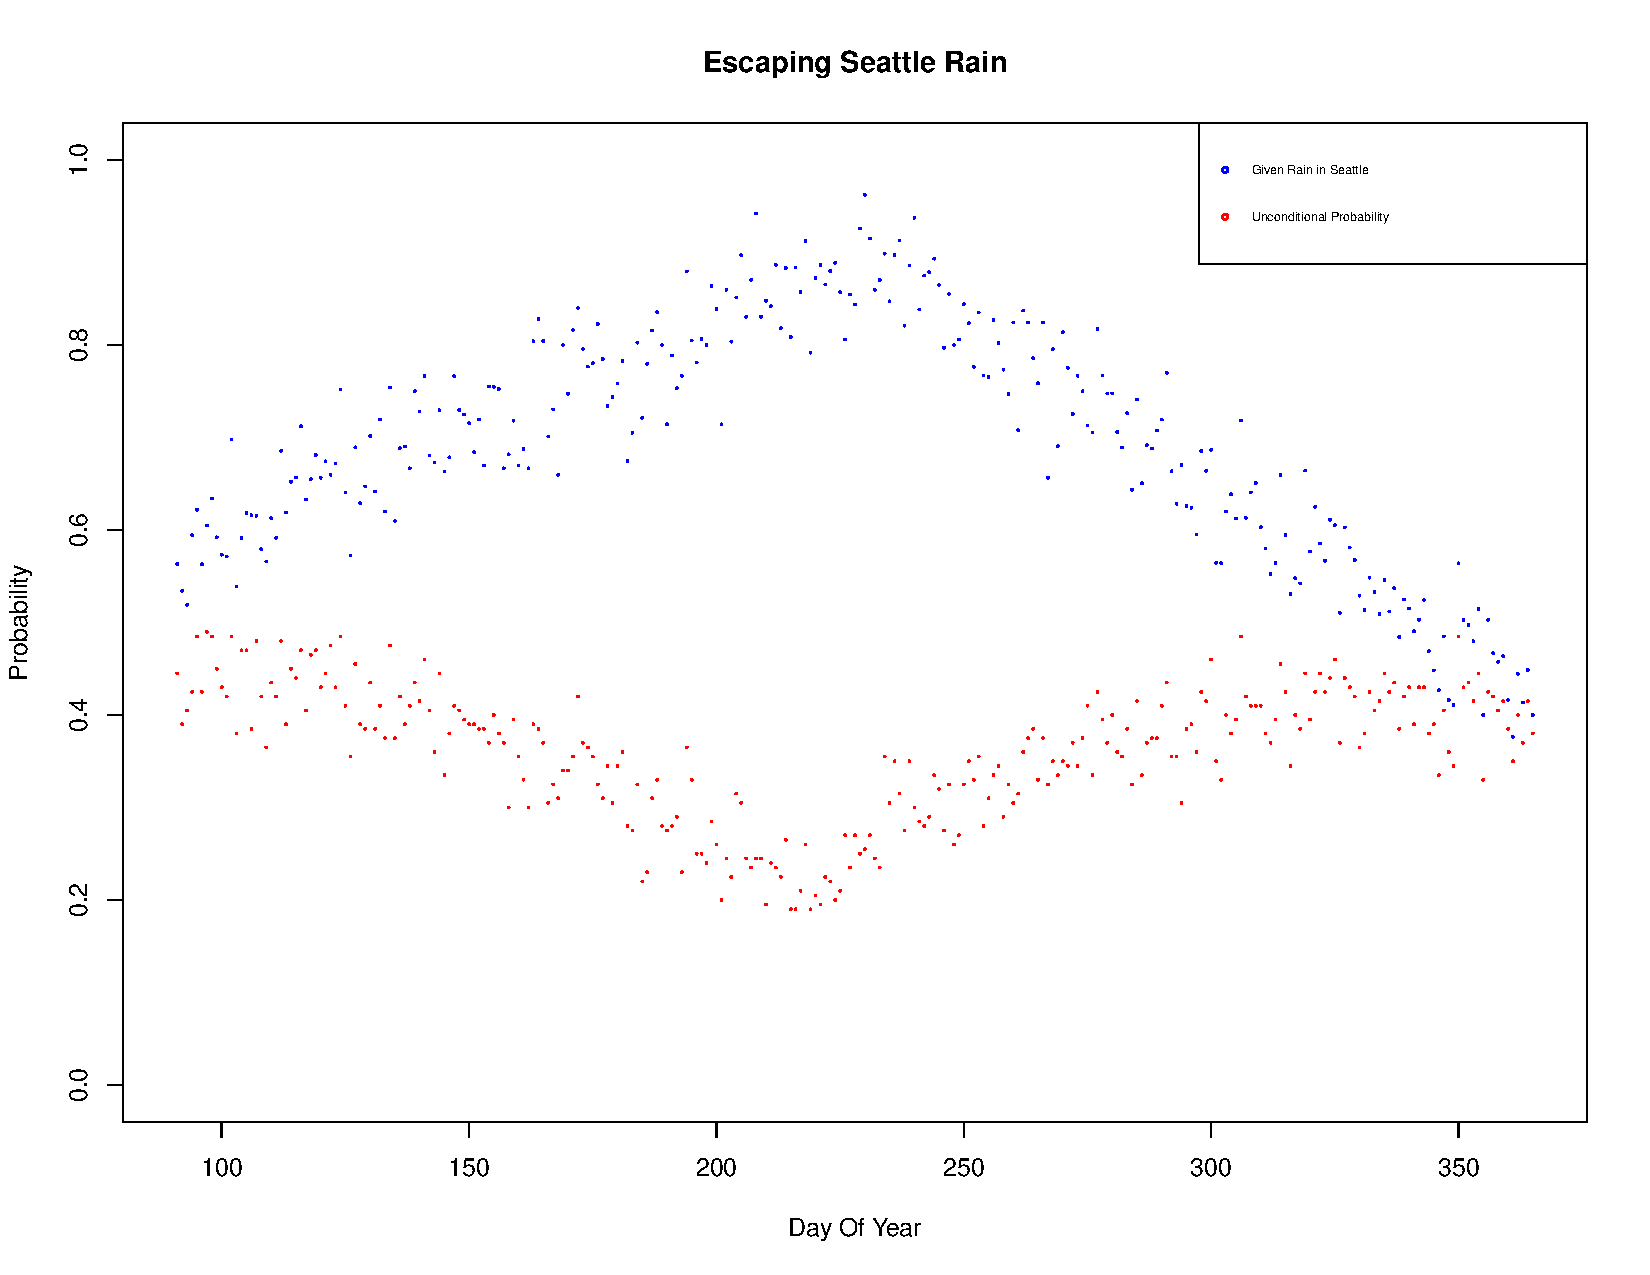
\includegraphics[width = .6\textwidth, height = 10cm]{Model2EscapeSeattleRain}
\caption{Daily chance of escaping precipitation in Seattle. In blue, is the probability that that Region 6 will be dry given that Region 3 rains. In red, is the probability that Region 3 is rainy and Region 6 is dry}
\label{fig:m2EscapeSeattle}
\end{figure}

Furthermore, we use this model to analyze the possibility of leaving the wet Seattle (region 3) climate for the drier climate to the east of the Cascade Mountains (region 6). These results are found in Figure \ref{fig:m2EscapeSeattle}, which maintains the V shape of the model. We find that during the summer, the chance of escaping Seattle rain is high if it rains, but such a need is rare because Seattle is dry as well in the summer. 
However, if one takes the perspective of a resort manager in the drier region, outside of the summertime, the chance of an influx of business from Seattle residents searching for drier weather is approximately constant. There is a balance between the higher demand from Seattle because of the increased chance of precipitation in the west and the leaving of the clientele because of the increased chance of precipitation in the drier climate as well.

This piecewise linear model gives additional insight into how the probability of precipitation changes throughout the year. It confirms the conclusion of the multivariate normal model outline in section 3.1, and shows how precipitation data of this sort yields the conclusions of the simpler model. 

\section{Conclusion}

In this report, we analyzed the precipitation in the Pacific Northwest by diving the area into 9 distinct regions and using 46 years of data with 30km by 30km resolution to approximate the region-wide precipitation.
Two models were proposed to understand how the chance of precipitation changes over the year. In the first, we divide the year into a rainy season and a dry season, and model the changeover point as a proxy for residents' experience with the weather patterns. 
Based on observed data, we proposed a semi-conjugate multivariable normal model for the changeover points. There was some correlation within regions, but assumed independence between regions. Subtle correlation between the regions, and within smaller subregions may be an avenue for further exploration with this data set.
Within this model, we also explored how the duration of the dry season varied across the regions. The Oregon Coast and Cascade mountains had the longest dry season, and we suggested that this is due to the large difference between the winter and summer in precipitation chance, so even moderately dry weather is classified as the dry season. 
The second model we proposed seeks to understand how the probability of precipitation changes throughout the year on a daily level, as opposed to describing broad yearly climatic patterns. This model proposes a constant rate of decrease in the probability of precipitation during the springtime, and also a constant rate of increase during autumn, with some minimum chance of rain in the summer.
In this model, we found that the driest days of the year are earlier on western regions of the Pacific Northwest, however the eastern regions are drier overall, and also have a much drier summer. We also examined the opportunity for Seattle residents to escape rainy weather by traveling a short distance to the Columbia Plateau, and the model validates the tourism industry in the Columbia Plateau targeting Seattle residents. 

These models could be extended to include local measures of correlation, and to find in which areas is precipitation locally correlated, and which neighboring areas have low correlation. For example, in the 100 miles east of Seattle, there are 3 distinct climatic areas, which likely have low correlation, however 100 miles of coastline may be strongly correlated.
Further investigation is warranted into the weather patterns that cause all the regions east of the Cascade range to have a later driest day, and relatively drier weather later into the fall.




 
\end{document}